

\subsection{Соединения с водородными связями}

Водородные связи представляют собой один из видов невалентного взаимодействия, ведущего к притяжению. Среди всех видов такого притяжения, после ион-дипольных
взаимодействий, водородные связи - самые сильные. Но сравнению с ковалентными взаимодействиями, они, конечно, очень слабы (в среднем, 8-40 кДж/моль).

В водородной связи принимает участие атом водорода, уже связанный ковалентной связью с электроотрицательным атомом. Такая группа из двух атомов взимодействует с другим (или
таким же) высокоотрицательным атомом. Таким атомом может быть азот, кислород или фтор (хотя, к примеру, в газовой фазе в димере сероводорода тоже есть очень слабая водородная
связь).

Графически водородную связь изображают точками, чтобы подчеркнуть невалентность взаимодействия (рис. 1)

Важными особенностями строения является то, что угол Э-Н-Э всегда, если этому ничего не препятствует, старается установиться на 180 градусов. Однако можно получить и соединения
с уголковыми водородными связями, как на рис. 2: в этом случае в молекула может выбрать внутримолекулярную связь, а не связь с соседней молекулой. Еще одним примером будет
димер HF или H2O в газовой фазе (рис. 3): водородная сязь будет искажена из-за диполь-дипольного взаимодействия. Получается, что уголковые водородные связи образуются только
«искусственно», когда нет выбора. 

Также надо подчеркнуть, что атомы водорода, находящиеся между двумя связями, могут менять свои позиции, то есть мы имеем дело с динамическими системами. При этом,
посередине между двумя атомами есть энергетический барьер, поэтому там водород самопроизвольно находиться не может. От величины этого барьера зависит то, насколько часто и
быстро будут происходить переходы из одной формы в другую. График модели энергетического ящика на рис. 4. 

Заметим, что ион $F-H-F^-$ - не может быть рассмотрен в рамках представления о водородных связях. Во-первых, он симметричный, то есть водород сидит ровно посередине между
атомами фтора. Во-вторых, энергия связи значительно больше энергии водородной связи. В-третьих, расстояние между атомами фтора принципиально короче водородной связи.

В водородную связь более $80\%$ вносит вклад кулоновское взаимодействие. Поэтому, например, ассоциат молекулы аммиака с водой будет выглядеть, как на рис. 5, а не как на рис. 6,
ведь в первой структуре атом водорода на молекуле воды будет иметь больший частично положительный заряд, чем атом водорода у аммиака во второй структуре.

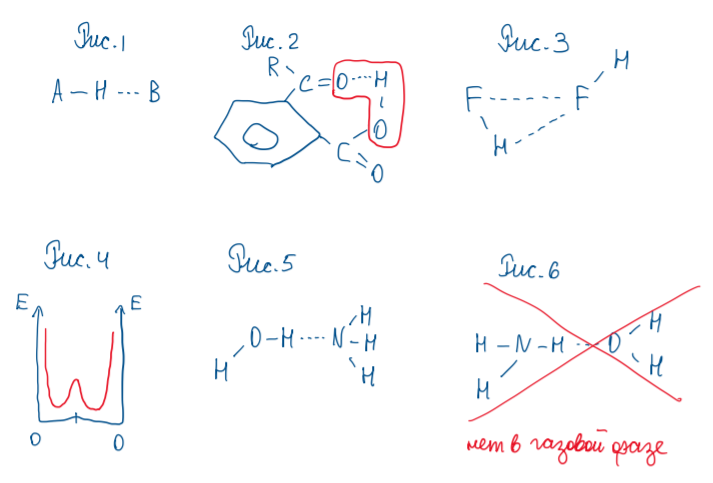
\includegraphics{images/17v1.png}

Наличие водородной связи сильно влияет на физические параметры вещества. У соединений, где характерны водородные связи (NH3, HF, H2O) наблюдается аномально высокие
температуры плавления и кипения, по сравнению с их аналогами. Более того, сильно увеличивается значение диэлектрической проницаемости вещества. Такие соединения очень
хорошо растворяют полярные соединения.

На молекулярном уровне наличие водородной связи ведёт к снижению расстояний между атомами по сравнению с суммой значений ван-дер-ваальсовых радиусов, что говорит о
некотором химическом связывании, а не простом сближении атомов. Например, в кристаллической решетки фтора расстояние между двумя молекулами фтора будет больше, чем
расстояние F-H-F, а расстояние O-H-O для водородной связи воды короче, чем сумма двух ван-дер-ваальсовых радиусов кислорода.

Важную роль водородная связь играет в структуре льда. Существует большое количество различных кристаллических модификаций льда, но выяснено, что независимо от их
кристаллической структуры все молекулы воды образуют связи друг с другом, участвует в этом каждый из атомов в молекуле воды. Во льду энергия одной водородной связи равна
примерно 20 кДж/моль. В газовой фазе энергия водородной связи меняется из-за иной геометрии (образуются ассоциаты - димеры).

HF в газовой фазе, помимо димеров, может давать и циклические олигомеры (рис. 7)

Удобным объектом для рассмотрения водородных связей являются карбоновые кислоты. Многие из них кристаллизуются с образованием димеров (рис. 8) и затем упаковываются в
кристаллическую решётку. Примечательно, что расстояние О-Н-О такое же, как в воде, и водород тоже не локализован в одном месте и постоянно перемещается от одного атома
кислорода к другому (рис.9)

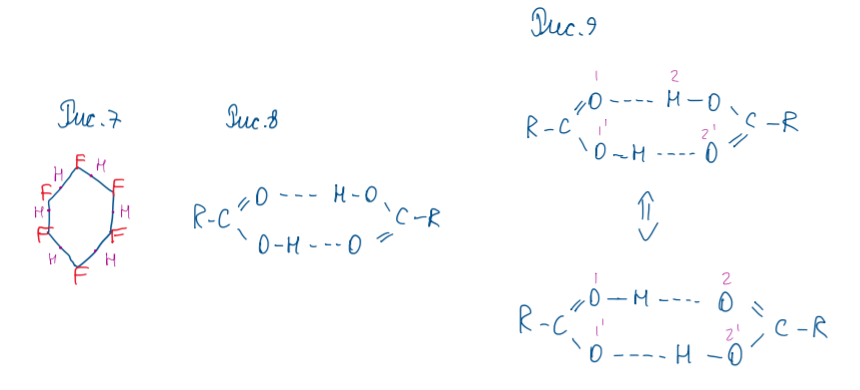
\includegraphics{images/17v2.png}
